\subsubsection{usergoal-ugCheckRequest}

\label{RE-use-case-ugCheckRequest}


The goal is to compare the new potential point of interest 
to the existing PIs in the system.		  


\begin{usecase}
  \addheading{Use-Case Description}
  \addsingletwocolumnrow{Name}{ugCheckRequest}
  \addsingletwocolumnrow{Scope}{system}
  \addsingletwocolumnrow{Level}{usergoal}
  

\addrowheading{Primary actor(s)}
\addnumberedsinglerow{}{\msrcode{actCoordinator[active]}}



\addrowheading{Goal(s) description}
\addsinglerow{The goal is to compare the new potential point of interest 
to the existing PIs in the system.}

\addrowheading{Reuse}
\addnumberedsinglerow{}{\msrucname{ugSecurelyUseSystem [1..1]}}
\addnumberedsinglerow{}{\msrucname{oeGetAllRequests [1..1]}}
\addnumberedsinglerow{}{\msrucname{oeCheckAvailability [1..*]}}
\addnumberedsinglerow{}{\msrucname{oeDeliverRequest [1..*]}}

\addrowheading{Protocol condition(s)}
\addnumberedsinglerow{}{
the iCrash system has been deployed
}

\addrowheading{Pre-condition(s)}
\addnumberedsinglerow{}{
none
}

\addrowheading{Main post-condition(s)}
\addnumberedsinglerow{}{
there exist one request whose ignored information has been changed.
}

\addrowheading{Main Steps}
\addalphanumberedsinglerow{}{the actor \msrcode{actCoordinator} executes the \msrucname{ugSecurelyUseSystem} use case}
\addalphanumberedsinglerow{}{the actor \msrcode{actCoordinator} executes the \msrucname{oeGetAllRequests} use case}
\addalphanumberedsinglerow{}{the actor \msrcode{actCoordinator} executes the \msrucname{oeCheckAvailability} use case}
\addalphanumberedsinglerow{}{the actor \msrcode{actCoordinator} executes the \msrucname{oeDeliverRequest} use case}
\addrowheading{Steps Ordering Constraints}
\addnumberedsinglerow{}{step (a) must always be performed before all the other steps.}
\addnumberedsinglerow{}{Subsequently, all the steps follow after step (a) is performed.}

\addrowheading{Additional Information}
\addsinglerow{
none
}

\end{usecase} 


Figure \ref{fig:lu.uni.lassy.excalibur.MyCrash.G02-RE-UCD-uc-ugCheckRequest}
The coordinator checks if the requested point of interest is not already in the system.

\begin{figure}[htbp]
\begin{center}

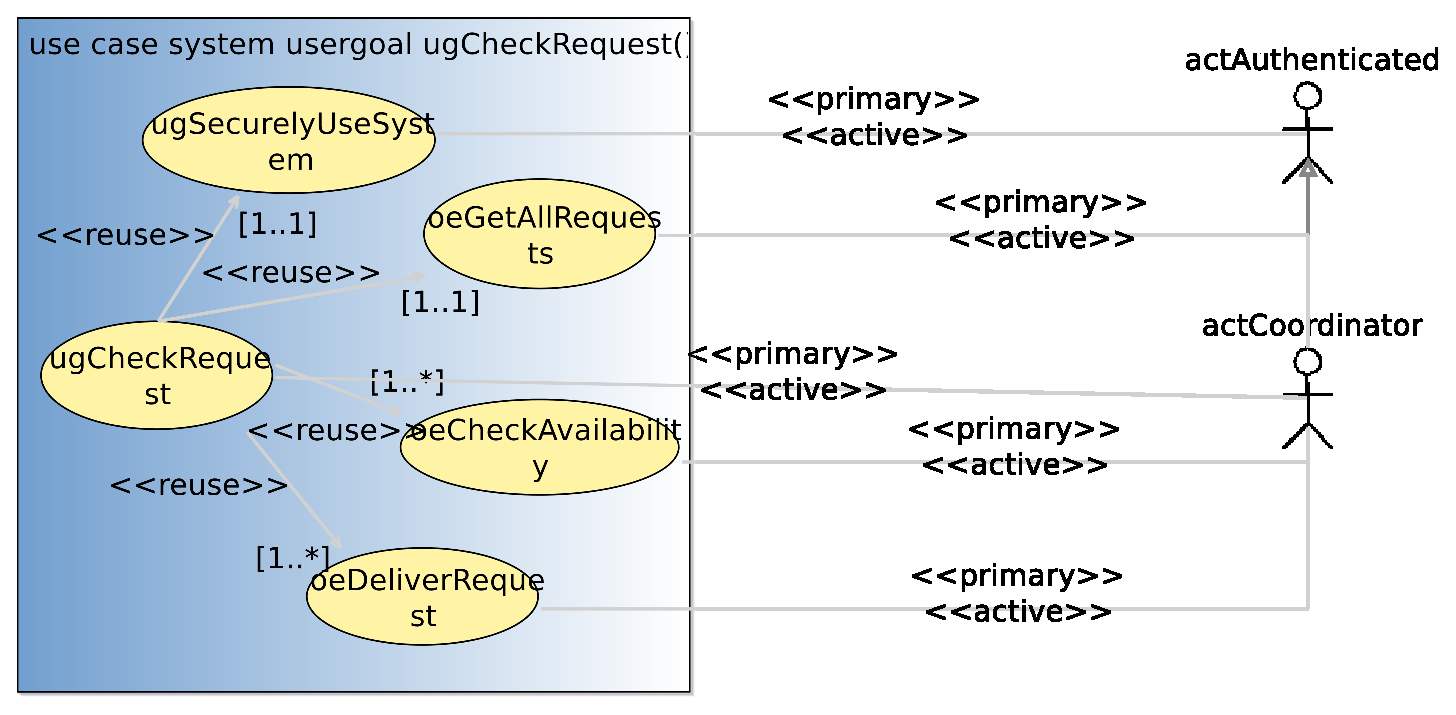
\includegraphics[
angle=0
,width=1.0\textwidth
]{./images-report-gen/usecase-model/usergoal/uc-ugCheckRequest.eps}
\end{center}
\caption[lu.uni.lassy.excalibur.MyCrash.G02 Use Case Diagram: uc-ugCheckRequest]{ugCheckRequest user goal use case}
\label{fig:lu.uni.lassy.excalibur.MyCrash.G02-RE-UCD-uc-ugCheckRequest}
\end{figure}
\vspace{0.5cm}
